\section{Calibration and commissioning}
\subsection{Prototyping}
Two prototypes of the FT-Cal, with 9 and 16 channels respectively, have been assembled and tested with cosmic rays and electron beams. The prototypes were used to check 
the single crystal mechanical assembly, the thermal performance, the front-end and read-out electronics, 
the electrical connections via a motherboard.
The response to cosmic rays was studied for both prototypes while the response to electromagnetic shower was studied at JLab and LNF.
The Proto-9 has been  tested at JLab using 2-3 GeV
electrons deviated by the Hall-B tagger system  while the Proto-16 has been tested at the Beam Test Facility of LNF with a 0.7 GeV electron beam.  Extensive simulations have been performed and compared to the results of the two sets of measurements. 
Main goals of  tests were:

\begin{figure}
\includegraphics[width=1.0\columnwidth]{./fig/p9-whole.eps}
\caption{FT-Cal Proto-9 full assembly.}
\label{fig:p9-whole}
\end{figure}

\begin{itemize}
\item to measure the energy resolution as a function of single-crystal threshold;
\item to measure the energy resolution as a function of T (+18$^\circ$, 0$^\circ$, -10$^\circ$, -25$^\circ$);
\item to measure the time resolution;
\item to verify the system linearity;
\item to check rate performances;
\item to validate GEMC simulations;
\item to measure the electronic noise in realistic conditions;
\item to perform detailed studies of electromagnetic shower signal: shower profile, APD signal shape, and test of filtering algorithm.
\end{itemize}

\subsubsection{The Proto-16}\label{par:proto-16}
The FT-Cal Proto-16, was built assembling
16 crystals in a $4\times4$ matrix (8 provided by the BTCP and 8 from
the RIINC company).
Figure~\ref{fig:p16-whole} shows the Proto-16
components.  
Many mechanical and electrical solutions tested on Proto-16 were then adopted in the final FT-Cal design.
\begin{figure}
\includegraphics[width=1.0\columnwidth]{./fig/p16-whole.eps}
\caption{Exploded view of the Proto-16 assembly}
\label{fig:p16-whole}
\end{figure}
Due to a significant size of the  crystal matrix the expected performance of Proto-16 in terms of energy resolution are similar to what expected for the the FT-Cal. 
The Proto-16 was tested at the Beam Test Facility (BTF) \cite{btf} of
the INFN Frascati National Laboratory, using a 500 MeV electron
beam. Data were taken in  October 2012 studying  the prototype
resolution as a function of the energy and calorimeter temperature. The BTF electron beam is characterized a repetition
frequency of 50 Hz and a pulse duration of 10 ns. The beam intensity
can be varied by operating different sets of slits, selecting the
number of electrons per bunch at the level of a single particle. The
prototype performance can therefore be studied as a function of the
number of electrons hitting simultaneously the crystal matrix, i.e. of
the detected energy.


Fig. \ref{fig:btf} shows the experimental hall after the installation
of the Proto-16 and associated equipment. The detector was placed on a
moveable table that can be displaced in the x and y direction with
0.1-mm accuracy. This feature was exploited to center the calorimeter
with respect to the beam. A plastic scintillator bar, read by two
PMTs, was placed in front of the beam pipe exit window and was used to
determine the arrival time of the electron within the 10-ns bunch
duration. The data acquisition, based on the JLAB DAQ standard CODA,
was triggered by the RF signal of the Frascati accelerator. For each
trigger all the signals of the Proto-16 crystal matrix and of the
scintillator-bar PMTs were recorded by CAEN VME boards. Both the
Proto-16 and scintillator signals were sent to a passive splitter
whose two outputs were connected the 250 MHz fADCs and to leading-edge
discriminators. The discriminator output was sent to pipeline
TDCs. The samples recorded by the fADCs in a 800 ns window were recorded for
each trigger and analyzed offline to evaluate the charge and time.

\begin{figure}
\includegraphics[width=1.0\columnwidth]{./fig/btf_oct12.eps}
\caption{Experimental setup in October Proto-16 test at the Frascati Beam Test Facility (BTF).}
\label{fig:btf}
\end{figure}

The conversion between charge and energy  was first determined using cosmic ray measurements and  then
optimized  by studying the response of each crystal
to 500 MeV electrons at the LNF-BTF. It worth noticing that the new calibration constants were
found to be within 5-10\% from the initial values determined with the
cosmic-ray data taking.
The total reconstructed energy  after
the full calibration is shown in Fig.~\ref{fig:btf_etot} for an
electron multiplicity of the order of 1-2. The peaks corresponding to
different bunch population are clearly visible and well
separated. 
\begin{figure}
\includegraphics[width=1.0\columnwidth]{./fig/btf_etot_1876_2_6.eps}
\caption{The  total energy measured by Proto-16 after 
  calibration.Peaks corresponding to different
  bunch population are clearly visible and well separated. }
\label{fig:btf_etot}
\end{figure}

\begin{figure}
\includegraphics[width=1.0\columnwidth]{./fig/btf_linearity_1876_2_6.eps}
\caption{Proto-16 reconstructed energy as a function of the beam bunch
  energy. The red points were obtained at room temperature and with a
APD gain of 150. The linear regression of the experimental points show
no deviation from linearity.}
\label{fig:btf_linearity}
\end{figure}

\paragraph{Energy resolution}

The mean values and $\sigma$ of the peaks in the total reconstructed
energy spectrum were analyzed to check the system linearity and
determine the resolution. The measurements were performed by centering
the beam on the calorimeter to have the maximum containment of the
electromagnetic shower. 
Fig.~\ref{fig:btf_linearity} shows the fitted
peak position as a function of total energy in the beam bunch for APD
gain of 150 and PbWO temperature of $18^{\circ}$. The linear
regression of the experimental points show no deviations from
linearity in the explored range. The same measurement performed in
different configurations gave consistent results, confirming that the
system is linear up to the maximum measured energy of 4 GeV.

Fig.~\ref{fig:btf_resolution} shows the energy resolution as a
function of the energy in the beam bunch. The colored points
correspond to the resolution measured with the Proto-16 while the
black open circle are the results of the GEMC simulations. The error
bars in the graph show the statistical uncertainty while the
systematic uncertainty was estimated to be in the order of 5\%. 
As expected, the experimental resolution increases for increasing energy,
reaching an asymptotic behavior at about 3 GeV. The measurements
performed in different configuration are in general consistent,
varying within a range of 0.5\% except for the resolution obtained at
room temperature and G=75 (orange points).
The resolution in this case is systematically worse then what obtained
at the same temperature but G=150. This was interpreted as
due to the preamplifier noise being the dominant factor in determining
the resolution at this temperature. From this we concluded that
working at high APD gain is the preferable configuration. 
\begin{figure}
\includegraphics[width=1.0\columnwidth]{./fig/btf_resolution.eps}
\caption{Proto-16 energy resolution  as a function of the beam bunch
  energy. The red and orange points were obtained at room temperature
  for an APD gain of 150 and 75, respectively. The green points
  correspond to $o^\circ$ degrees; the darker points were obtained
  removing the passive splitter. The blue and dark-blue points
  correspond to $-20^\circ$ with APD gain of 150 and 75,
  respectively. The open black circle show the expected resolution
  based on GEMC simulations. Only statistical errors are shown.}
\label{fig:btf_resolution}
\end{figure} 

The comparison of the resolution obtained at different temperature
show that lower temperatures, corresponding to higher light yield and
therefore larger signal, give better resolution. The best values were
obtained at $-20^{\circ}$, where the experimental points are in good
agreement with the simulation results. The dependence of the
resolution on the temperature is more evident for high bunch energies,
where threshold effects are smaller. Above 2 GeV, the resolution at
room temperature seems to be systematically higher than the one
obtained at $0^\circ$ or $-20^\circ$ with a difference of about
0.5\%. The difference of the resolution obtained at $0^\circ$ and $-20^\circ$ 
is on the contrary quite small and negligible within the systematic
errors. Based on this results and considering the technical
difficulties in operating the FT-Cal at very low temperature, we
concluded that the optimal operating temperature of the calorimeter is
$0^\circ$.

\subsection{Cosmic ray calibration}
\subsection{On-beam calibration}
